\section{Fantastic Joules and Where to Find Them}

\subsection{Introduction} 
The Internet was estimated, in 2022, to compose 1\% to 1.5\% of the global electricity consumption \cite{NetPerc}. 
At world scale, this consumption is far from negligible as the world's global consumption was estimated between \qty{24 000}{\tera\watt\hour} and \qty{26 000}{\tera\watt\hour}. 
This mean that, even though the Internet's proportion could seem small it is roughly equivalent to the estimated consumption of a reasonably developed country (like Spain with which is estimatedé around \qty{240}{\tera\watt\hour} \cite{NetPerc}). 

To reduce the Internet's energy consumption, it is necessary to properly understand what drives its energy demand.
In this section, we explore an article \cite{FantasticJoul} investigating the energy demand of internet routers
\footnote{The term router is used throughout this section to denote "wired network devices" including switches but excluding wireless access points and home routers.}.
To this end, it explores multiples ways to retrieve and estimate their power consumption. 

First, power data is retrieved in routers datasheets where "Typical" and "Maximum" power consumption estimations figure.
Those datasheets are mainly intended for network operators to dimension the power supply of a rack of servers or server room. 
Hence, they are estimated to be an overestimation of the actual power consumption of a deployed router.  
An interesting finding is that, sometimes, datasheets aren't only imprecise or overestimating but underestimating actual power consumption.  

Second, measurements on deployed hardware's power consumption are used. 
To do so, power supply units (PSU) are queried for their consumption measurements using standardized MIB objects over the simple network management protocol (SNMP) \cite{snmprfc}.
Those PSU measurements are compared with external measurements of the measured routers of the measured routers.

The last method relies on modeling the power consumption of deployed routers as proposed by \cite{35} with additional considerations for transceivers. 

From the explored methods research questions emerges :
\begin{enumerate}
	\item [\textbf{Q1)}] Are datasheets representative of actual power consumption ? 
	\item [\textbf{Q2)}] Are PSU measurements reliable ?
	\item [\textbf{Q3)}] Is it possible to precisely model deployed router power consumption ? 
\end{enumerate}

\todo[inline]{introduce sections and explain the 3 dataset combined}


\subsection{Datasheet extraction}\label{sec:datasheet} 
In this section, two objectives are pursued :
The first is to collect a set of power data of numerous router models from their datasheets.    
Once such dataset is formed, the second objective is to assess if datasheet are reliable.

The collection should be automated and if possible contain the following information :   
\begin{itemize}
	\item Maximum and typical power draw
	\item Number and capacity of PSU
	\item Maximum bandwidth
	\item Release, end-of-sale and end-of-support dates 
\end{itemize}
Although, router datasheets are publicly available online, the automation process is not straightforward. 
Since datasheets are organized differently, unstructured and, in some cases, incomplete.   
Moreover, one needs a list of routers and their associated datasheets to automate the collection. 

The solution used by the authors is a combination of an open-source device library \cite{NetBoxLib} used by NetBox, a network management software, and the GPT-o4 LLM. 
The former is used to collect a router list with their corresponding datasheets and their PSU information if present, and the latter is used to extract the actual data from the datasheets.
The manual assessment of the extracted data showed that the accurately was reasonably correct, even though, as one may imagine, not perfect. 
Figure \ref{fig:pipeline} illustrates the actual data parsing pipeline used by the article.

\begin{figure}
	\begin{center}
		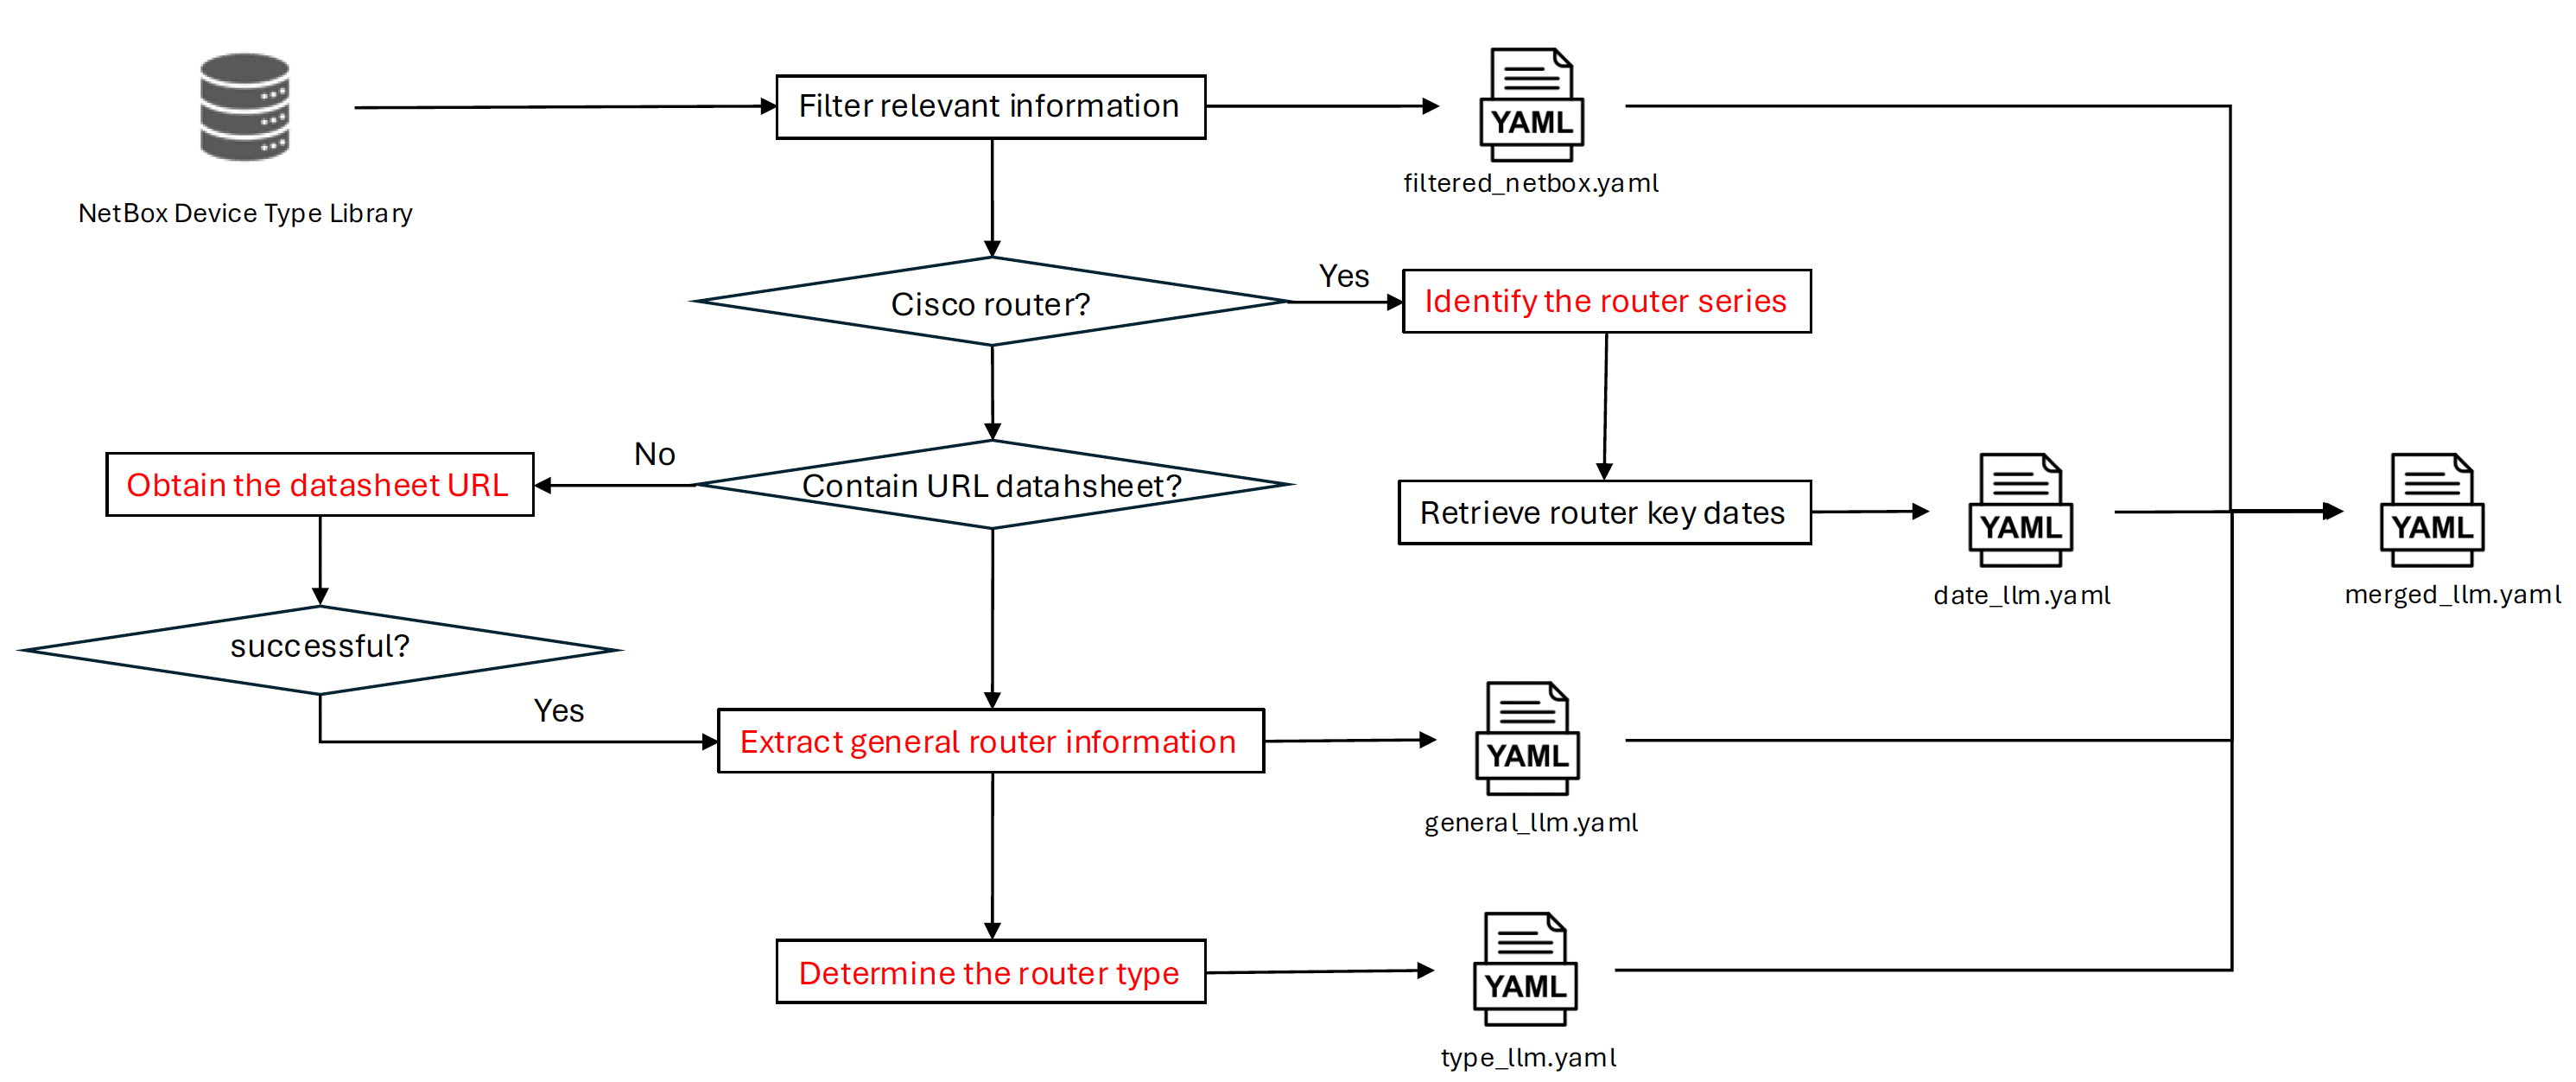
\includegraphics[width=0.95\columnwidth]{figures/data_parsing_pipeline.png}
	\end{center}
	\caption{The data parsing pipeline \cite{LLMpipe}. Red text highlights steps assisted by the LLM.}\label{fig:pipeline}
\end{figure}

The dataset is formed, using the explained methodology, of 777 router models data from Cisco, Arista and Juniper. 

\improvement[inline]{j'ai tendance à beaucoup les citer et utiliser leurs résultats mais n'ai pas trop le choix ?}

\subsection{Modeling and deriving parameters}\label{sec:model} 
The objective of the model is to be easily derivable and reproducible by operators with a similar setup as Autopower.
To this end, its parameters should be easily controllable and measurable.
The focus is aimed at networking effects such as link state or traffic volume.
Although other parameters may impact the actual power draw, such as temperature, OS version or fan speed, they are intentionally omitted to simplify reproducibility.

The power model is derived from a former article\cite{35}, the main contribution made is the addition of transceivers consideration. 
It is formed in a top-down manner and composed, on the highest level, of the static $P_{\textnormal{sta}}$ and dynamic $P_{\textnormal{dyn}}$ power draw.  
Both depend on a configuration vector $C$ that defines every interface configuration $c_i$, e.g. its throughput. 
The dynamic power also depends on the load vector L specifying the load at each interface $l_i$.
Therefore, the model can be written as : 
\begin{equation}
	P_{\textnormal{tot}} = P_{\textnormal{sta}}(C) + P_{\textnormal{dyn}}(C,L)
\end{equation}

First, to refine the static component of the model it is separated in $P_{\textnormal{base}}$, the power draw when the device is on without, and $P_{interface}$, the power draw per interface with respect to its configuration which should be summed for each interface. 
The latter can be refined in two terms $P_{port}$, the power consumed by the router interface port, and $P_{trx}$, the power consumed by the transceiver which is a pluggable module inserted to the port. 
Furthermore, empirical observation permits to write $P_{trx}$ as the sum of two terms $P_{trx,in}$, the power drawn when the transceiver is plugged in but off and $P_{trx,up}$, the power consumption when the interface is up.
Thus, the static component can be written

\begin{equation}
	P_{\textnormal{sta}}(C) = P_{\textnormal{base}}(C) + \sum_{i=0}^{N_{\textnormal{port}}}  P_{\textnormal{interface}}(c_i)
\end{equation}

\begin{equation}
	P_{\textnormal{interface}}(c_i) = P_{\textnormal{port}}(c_i) + P_{\textnormal{trx}}(c_i)
\end{equation}

\begin{equation}
	P_{\textnormal{trx}}(c_i) = P_{\textnormal{trx,in}}(c_i) + P_{\textnormal{trx,up}}(c_i)
\end{equation}

Second, the dynamic power is composed of the sum of two components per port.

The first ($P_{\textnormal{dyn, port}}$) defines the dynamic power consumption of a port assuming transceiver power is independent of traffic load.
It can be further decomposed by the energy necessary to process a bit $E_\textnormal{bit}$ (resp. a packet $E_\textnormal{pkt}$) multiplied by the bit (resp. packet) rate $r_i$ (resp. $p_i$).

The second is $P_\textnormal{offset}$ which is independent of traffic and added to preserve the linear behaviour of the dynamic power consumption empirically.
In no traffic situation, some device have a considerable power difference, either positive or negative, to the expected linear behaviour. 
Concretely, this power offset is the difference between no traffic and (very) low traffic scenarios.  
Keeping the linear behaviour later helps to derive the model parameters. 

However, a missing piece still remains in the understanding of this offset. 
Although a positive offset could be explained by the fact that, in no traffic scenarios, routers may optimize the power consumption of components.
Thus, reducing the actual power draw resulting in a positive offset.  
The scenario of a negative offset is still unexplained as stated by Lin Jackie in its thesis\cite{lim} "it is unclear to us where this negative offset comes from. One speculation is that this behaviour is device-specific and may only occur on Cisco devices, and therefore depends on the circuit design of the device." 

Regardless, the dynamic power component expressed

\begin{equation}
	P_{\textnormal{dyn}}(C,L) = \sum_{i=0}^{N_\textnormal{port}} P_{\textnormal{dyn,port}}(c_i,l_i) + P_\textnormal{offset}(c_i)
\end{equation}

\begin{equation}
	P_{\textnormal{dyn,port}}(c_i,l_i) = E_\textnormal{bit}(c_i) \cdot r_i + E_\textnormal{pkt}(c_i) \cdot p_i 
\end{equation}

This gives a model where only 4 parameters need to be derived : 


\todo[inline]{derivation}
mention Lin jackie's thesis  

\begin{figure}[ht]
	\begin{center}
		\includesvg[width=0.5\columnwidth]{figures/Snake.drawio.svg}
	\end{center}
	\caption{Illustration of the Snake as defined in RFC 8239\cite{rfc8239}.}\label{fig:}
\end{figure}



\subsection{PSU and external measurements}\label{sec:PSUExternal} 
The collection of power supply units measurements to address if they are grounded (\textbf{Q2}) is explained in the following.  
PSU and interface traffic measurements are made during a 10-months period with a \qty{5}{\min} interval between queries over 107 routers deployed in Switch\cite{SwitchISP}, a Tier-2 ISP.
The ISP serves as the National Research and Education Network (NREN) just, as Belnet is in Belgium. Thanks to its role, it is more incline to accept research project enabling the collection of those power measurements. 
The interface traffic measurements are collected to possibly correlate the amount of traffic and the power draw.

In addition to this collection, the authors collected external, PSU and traffic measurements during a 2-months period over 3 routers in the same ISP.  
This collection was made possible by Autopower\cite{Autopower}, a system composed of a Raspberry Pi 4 and a Microchip MCP39F511N power meter featuring two measurements channels.
This allows to measure externally the power draw of a router and power the Pi simultaneously.
Which is an interesting point because it doesn't require an additional power plug in the ISP facility, which are often times spares. 
The Pi controls the measurements samples of the Microchip and a client-server application built with gRPC to enable users to retrieve samples and control the measurements remotely.
Connecting the client to the server is done on the client side to permit the Autopower to work even behind a NAT.

The system is made to be easily reproducible and cheap for operators to measure their router power data.
Possibly sharing it to create a similar system to RIPE Atlas\cite{ripeAtlas} but for power measurements and not internet connectivity.

\subsection{Comparing power data sources}\label{sec:Fanresults} 
\todo[inline]{6 }

The first research question (\textbf{Q1}) can now be addressed using it.

\textit{Are datasheets reliable in power draw information ?}
Although, as discussed earlier, datasheets power values are meant to dimension racks or servers room, knowing if their typical power draw claims are accurate is addressed.  
To do so, 

\subsection{Insights in router power}\label{sec:insight} 
\todo[inline]{and 7, 8th and 9th (quickly mention it  stating it is only preliminary insight)}
\subsection{Towards improving Power consumption}\label{sec:improving} 
\todo[inline]{leverage insights to foster future research directions}
\subsection{Conclusion}\label{sec:conclusion} 

